\documentclass[crop=false,class=article,oneside]{standalone}
%----------------------------Preamble-------------------------------%
%---------------------------Packages----------------------------%
\usepackage{geometry}
\geometry{b5paper, margin=1.0in}
\usepackage[T1]{fontenc}
\usepackage{graphicx, float}            % Graphics/Images.
\usepackage{natbib}                     % For bibliographies.
\bibliographystyle{agsm}                % Bibliography style.
\usepackage[french, english]{babel}     % Language typesetting.
\usepackage[dvipsnames]{xcolor}         % Color names.
\usepackage{listings}                   % Verbatim-Like Tools.
\usepackage{mathtools, esint, mathrsfs} % amsmath and integrals.
\usepackage{amsthm, amsfonts, amssymb}  % Fonts and theorems.
\usepackage{tcolorbox}                  % Frames around theorems.
\usepackage{upgreek}                    % Non-Italic Greek.
\usepackage{fmtcount, etoolbox}         % For the \book{} command.
\usepackage[newparttoc]{titlesec}       % Formatting chapter, etc.
\usepackage{titletoc}                   % Allows \book in toc.
\usepackage[nottoc]{tocbibind}          % Bibliography in toc.
\usepackage[titles]{tocloft}            % ToC formatting.
\usepackage{pgfplots, tikz}             % Drawing/graphing tools.
\usepackage{imakeidx}                   % Used for index.
\usetikzlibrary{
    calc,                   % Calculating right angles and more.
    angles,                 % Drawing angles within triangles.
    arrows.meta,            % Latex and Stealth arrows.
    quotes,                 % Adding labels to angles.
    positioning,            % Relative positioning of nodes.
    decorations.markings,   % Adding arrows in the middle of a line.
    patterns,
    arrows
}                                       % Libraries for tikz.
\pgfplotsset{compat=1.9}                % Version of pgfplots.
\usepackage[font=scriptsize,
            labelformat=simple,
            labelsep=colon]{subcaption} % Subfigure captions.
\usepackage[font={scriptsize},
            hypcap=true,
            labelsep=colon]{caption}    % Figure captions.
\usepackage[pdftex,
            pdfauthor={Ryan Maguire},
            pdftitle={Mathematics and Physics},
            pdfsubject={Mathematics, Physics, Science},
            pdfkeywords={Mathematics, Physics, Computer Science, Biology},
            pdfproducer={LaTeX},
            pdfcreator={pdflatex}]{hyperref}
\hypersetup{
    colorlinks=true,
    linkcolor=blue,
    filecolor=magenta,
    urlcolor=Cerulean,
    citecolor=SkyBlue
}                           % Colors for hyperref.
\usepackage[toc,acronym,nogroupskip,nopostdot]{glossaries}
\usepackage{glossary-mcols}
%------------------------Theorem Styles-------------------------%
\theoremstyle{plain}
\newtheorem{theorem}{Theorem}[section]

% Define theorem style for default spacing and normal font.
\newtheoremstyle{normal}
    {\topsep}               % Amount of space above the theorem.
    {\topsep}               % Amount of space below the theorem.
    {}                      % Font used for body of theorem.
    {}                      % Measure of space to indent.
    {\bfseries}             % Font of the header of the theorem.
    {}                      % Punctuation between head and body.
    {.5em}                  % Space after theorem head.
    {}

% Italic header environment.
\newtheoremstyle{thmit}{\topsep}{\topsep}{}{}{\itshape}{}{0.5em}{}

% Define environments with italic headers.
\theoremstyle{thmit}
\newtheorem*{solution}{Solution}

% Define default environments.
\theoremstyle{normal}
\newtheorem{example}{Example}[section]
\newtheorem{definition}{Definition}[section]
\newtheorem{problem}{Problem}[section]

% Define framed environment.
\tcbuselibrary{most}
\newtcbtheorem[use counter*=theorem]{ftheorem}{Theorem}{%
    before=\par\vspace{2ex},
    boxsep=0.5\topsep,
    after=\par\vspace{2ex},
    colback=green!5,
    colframe=green!35!black,
    fonttitle=\bfseries\upshape%
}{thm}

\newtcbtheorem[auto counter, number within=section]{faxiom}{Axiom}{%
    before=\par\vspace{2ex},
    boxsep=0.5\topsep,
    after=\par\vspace{2ex},
    colback=Apricot!5,
    colframe=Apricot!35!black,
    fonttitle=\bfseries\upshape%
}{ax}

\newtcbtheorem[use counter*=definition]{fdefinition}{Definition}{%
    before=\par\vspace{2ex},
    boxsep=0.5\topsep,
    after=\par\vspace{2ex},
    colback=blue!5!white,
    colframe=blue!75!black,
    fonttitle=\bfseries\upshape%
}{def}

\newtcbtheorem[use counter*=example]{fexample}{Example}{%
    before=\par\vspace{2ex},
    boxsep=0.5\topsep,
    after=\par\vspace{2ex},
    colback=red!5!white,
    colframe=red!75!black,
    fonttitle=\bfseries\upshape%
}{ex}

\newtcbtheorem[auto counter, number within=section]{fnotation}{Notation}{%
    before=\par\vspace{2ex},
    boxsep=0.5\topsep,
    after=\par\vspace{2ex},
    colback=SeaGreen!5!white,
    colframe=SeaGreen!75!black,
    fonttitle=\bfseries\upshape%
}{not}

\newtcbtheorem[use counter*=remark]{fremark}{Remark}{%
    fonttitle=\bfseries\upshape,
    colback=Goldenrod!5!white,
    colframe=Goldenrod!75!black}{ex}

\newenvironment{bproof}{\textit{Proof.}}{\hfill$\square$}
\tcolorboxenvironment{bproof}{%
    blanker,
    breakable,
    left=3mm,
    before skip=5pt,
    after skip=10pt,
    borderline west={0.6mm}{0pt}{green!80!black}
}

\AtEndEnvironment{lexample}{$\hfill\textcolor{red}{\blacksquare}$}
\newtcbtheorem[use counter*=example]{lexample}{Example}{%
    empty,
    title={Example~\theexample},
    boxed title style={%
        empty,
        size=minimal,
        toprule=2pt,
        top=0.5\topsep,
    },
    coltitle=red,
    fonttitle=\bfseries,
    parbox=false,
    boxsep=0pt,
    before=\par\vspace{2ex},
    left=0pt,
    right=0pt,
    top=3ex,
    bottom=1ex,
    before=\par\vspace{2ex},
    after=\par\vspace{2ex},
    breakable,
    pad at break*=0mm,
    vfill before first,
    overlay unbroken={%
        \draw[red, line width=2pt]
            ([yshift=-1.2ex]title.south-|frame.west) to
            ([yshift=-1.2ex]title.south-|frame.east);
        },
    overlay first={%
        \draw[red, line width=2pt]
            ([yshift=-1.2ex]title.south-|frame.west) to
            ([yshift=-1.2ex]title.south-|frame.east);
    },
}{ex}

\AtEndEnvironment{ldefinition}{$\hfill\textcolor{Blue}{\blacksquare}$}
\newtcbtheorem[use counter*=definition]{ldefinition}{Definition}{%
    empty,
    title={Definition~\thedefinition:~{#1}},
    boxed title style={%
        empty,
        size=minimal,
        toprule=2pt,
        top=0.5\topsep,
    },
    coltitle=Blue,
    fonttitle=\bfseries,
    parbox=false,
    boxsep=0pt,
    before=\par\vspace{2ex},
    left=0pt,
    right=0pt,
    top=3ex,
    bottom=0pt,
    before=\par\vspace{2ex},
    after=\par\vspace{1ex},
    breakable,
    pad at break*=0mm,
    vfill before first,
    overlay unbroken={%
        \draw[Blue, line width=2pt]
            ([yshift=-1.2ex]title.south-|frame.west) to
            ([yshift=-1.2ex]title.south-|frame.east);
        },
    overlay first={%
        \draw[Blue, line width=2pt]
            ([yshift=-1.2ex]title.south-|frame.west) to
            ([yshift=-1.2ex]title.south-|frame.east);
    },
}{def}

\AtEndEnvironment{ltheorem}{$\hfill\textcolor{Green}{\blacksquare}$}
\newtcbtheorem[use counter*=theorem]{ltheorem}{Theorem}{%
    empty,
    title={Theorem~\thetheorem:~{#1}},
    boxed title style={%
        empty,
        size=minimal,
        toprule=2pt,
        top=0.5\topsep,
    },
    coltitle=Green,
    fonttitle=\bfseries,
    parbox=false,
    boxsep=0pt,
    before=\par\vspace{2ex},
    left=0pt,
    right=0pt,
    top=3ex,
    bottom=-1.5ex,
    breakable,
    pad at break*=0mm,
    vfill before first,
    overlay unbroken={%
        \draw[Green, line width=2pt]
            ([yshift=-1.2ex]title.south-|frame.west) to
            ([yshift=-1.2ex]title.south-|frame.east);},
    overlay first={%
        \draw[Green, line width=2pt]
            ([yshift=-1.2ex]title.south-|frame.west) to
            ([yshift=-1.2ex]title.south-|frame.east);
    }
}{thm}

%--------------------Declared Math Operators--------------------%
\DeclareMathOperator{\adjoint}{adj}         % Adjoint.
\DeclareMathOperator{\Card}{Card}           % Cardinality.
\DeclareMathOperator{\curl}{curl}           % Curl.
\DeclareMathOperator{\diam}{diam}           % Diameter.
\DeclareMathOperator{\dist}{dist}           % Distance.
\DeclareMathOperator{\Div}{div}             % Divergence.
\DeclareMathOperator{\Erf}{Erf}             % Error Function.
\DeclareMathOperator{\Erfc}{Erfc}           % Complementary Error Function.
\DeclareMathOperator{\Ext}{Ext}             % Exterior.
\DeclareMathOperator{\GCD}{GCD}             % Greatest common denominator.
\DeclareMathOperator{\grad}{grad}           % Gradient
\DeclareMathOperator{\Ima}{Im}              % Image.
\DeclareMathOperator{\Int}{Int}             % Interior.
\DeclareMathOperator{\LC}{LC}               % Leading coefficient.
\DeclareMathOperator{\LCM}{LCM}             % Least common multiple.
\DeclareMathOperator{\LM}{LM}               % Leading monomial.
\DeclareMathOperator{\LT}{LT}               % Leading term.
\DeclareMathOperator{\Mod}{mod}             % Modulus.
\DeclareMathOperator{\Mon}{Mon}             % Monomial.
\DeclareMathOperator{\multideg}{mutlideg}   % Multi-Degree (Graphs).
\DeclareMathOperator{\nul}{nul}             % Null space of operator.
\DeclareMathOperator{\Ord}{Ord}             % Ordinal of ordered set.
\DeclareMathOperator{\Prin}{Prin}           % Principal value.
\DeclareMathOperator{\proj}{proj}           % Projection.
\DeclareMathOperator{\Refl}{Refl}           % Reflection operator.
\DeclareMathOperator{\rk}{rk}               % Rank of operator.
\DeclareMathOperator{\sgn}{sgn}             % Sign of a number.
\DeclareMathOperator{\sinc}{sinc}           % Sinc function.
\DeclareMathOperator{\Span}{Span}           % Span of a set.
\DeclareMathOperator{\Spec}{Spec}           % Spectrum.
\DeclareMathOperator{\supp}{supp}           % Support
\DeclareMathOperator{\Tr}{Tr}               % Trace of matrix.
%--------------------Declared Math Symbols--------------------%
\DeclareMathSymbol{\minus}{\mathbin}{AMSa}{"39} % Unary minus sign.
%------------------------New Commands---------------------------%
\DeclarePairedDelimiter\norm{\lVert}{\rVert}
\DeclarePairedDelimiter\ceil{\lceil}{\rceil}
\DeclarePairedDelimiter\floor{\lfloor}{\rfloor}
\newcommand*\diff{\mathop{}\!\mathrm{d}}
\newcommand*\Diff[1]{\mathop{}\!\mathrm{d^#1}}
\renewcommand*{\glstextformat}[1]{\textcolor{RoyalBlue}{#1}}
\renewcommand{\glsnamefont}[1]{\textbf{#1}}
\renewcommand\labelitemii{$\circ$}
\renewcommand\thesubfigure{%
    \arabic{chapter}.\arabic{figure}.\arabic{subfigure}}
\addto\captionsenglish{\renewcommand{\figurename}{Fig.}}
\numberwithin{equation}{section}

\renewcommand{\vector}[1]{\boldsymbol{\mathrm{#1}}}

\newcommand{\uvector}[1]{\boldsymbol{\hat{\mathrm{#1}}}}
\newcommand{\topspace}[2][]{(#2,\tau_{#1})}
\newcommand{\measurespace}[2][]{(#2,\varSigma_{#1},\mu_{#1})}
\newcommand{\measurablespace}[2][]{(#2,\varSigma_{#1})}
\newcommand{\manifold}[2][]{(#2,\tau_{#1},\mathcal{A}_{#1})}
\newcommand{\tanspace}[2]{T_{#1}{#2}}
\newcommand{\cotanspace}[2]{T_{#1}^{*}{#2}}
\newcommand{\Ckspace}[3][\mathbb{R}]{C^{#2}(#3,#1)}
\newcommand{\funcspace}[2][\mathbb{R}]{\mathcal{F}(#2,#1)}
\newcommand{\smoothvecf}[1]{\mathfrak{X}(#1)}
\newcommand{\smoothonef}[1]{\mathfrak{X}^{*}(#1)}
\newcommand{\bracket}[2]{[#1,#2]}

%------------------------Book Command---------------------------%
\makeatletter
\renewcommand\@pnumwidth{1cm}
\newcounter{book}
\renewcommand\thebook{\@Roman\c@book}
\newcommand\book{%
    \if@openright
        \cleardoublepage
    \else
        \clearpage
    \fi
    \thispagestyle{plain}%
    \if@twocolumn
        \onecolumn
        \@tempswatrue
    \else
        \@tempswafalse
    \fi
    \null\vfil
    \secdef\@book\@sbook
}
\def\@book[#1]#2{%
    \refstepcounter{book}
    \addcontentsline{toc}{book}{\bookname\ \thebook:\hspace{1em}#1}
    \markboth{}{}
    {\centering
     \interlinepenalty\@M
     \normalfont
     \huge\bfseries\bookname\nobreakspace\thebook
     \par
     \vskip 20\p@
     \Huge\bfseries#2\par}%
    \@endbook}
\def\@sbook#1{%
    {\centering
     \interlinepenalty \@M
     \normalfont
     \Huge\bfseries#1\par}%
    \@endbook}
\def\@endbook{
    \vfil\newpage
        \if@twoside
            \if@openright
                \null
                \thispagestyle{empty}%
                \newpage
            \fi
        \fi
        \if@tempswa
            \twocolumn
        \fi
}
\newcommand*\l@book[2]{%
    \ifnum\c@tocdepth >-3\relax
        \addpenalty{-\@highpenalty}%
        \addvspace{2.25em\@plus\p@}%
        \setlength\@tempdima{3em}%
        \begingroup
            \parindent\z@\rightskip\@pnumwidth
            \parfillskip -\@pnumwidth
            {
                \leavevmode
                \Large\bfseries#1\hfill\hb@xt@\@pnumwidth{\hss#2}
            }
            \par
            \nobreak
            \global\@nobreaktrue
            \everypar{\global\@nobreakfalse\everypar{}}%
        \endgroup
    \fi}
\newcommand\bookname{Book}
\renewcommand{\thebook}{\texorpdfstring{\Numberstring{book}}{book}}
\providecommand*{\toclevel@book}{-2}
\makeatother
\titleformat{\part}[display]
    {\Large\bfseries}
    {\partname\nobreakspace\thepart}
    {0mm}
    {\Huge\bfseries}
\titlecontents{part}[0pt]
    {\large\bfseries}
    {\partname\ \thecontentslabel: \quad}
    {}
    {\hfill\contentspage}
\titlecontents{chapter}[0pt]
    {\bfseries}
    {\chaptername\ \thecontentslabel:\quad}
    {}
    {\hfill\contentspage}
\newglossarystyle{longpara}{%
    \setglossarystyle{long}%
    \renewenvironment{theglossary}{%
        \begin{longtable}[l]{{p{0.25\hsize}p{0.65\hsize}}}
    }{\end{longtable}}%
    \renewcommand{\glossentry}[2]{%
        \glstarget{##1}{\glossentryname{##1}}%
        &\glossentrydesc{##1}{~##2.}
        \tabularnewline%
        \tabularnewline
    }%
}
\newglossary[not-glg]{notation}{not-gls}{not-glo}{Notation}
\newcommand*{\newnotation}[4][]{%
    \newglossaryentry{#2}{type=notation, name={\textbf{#3}, },
                          text={#4}, description={#4},#1}%
}
%--------------------------LENGTHS------------------------------%
% Spacings for the Table of Contents.
\addtolength{\cftsecnumwidth}{1ex}
\addtolength{\cftsubsecindent}{1ex}
\addtolength{\cftsubsecnumwidth}{1ex}
\addtolength{\cftfignumwidth}{1ex}
\addtolength{\cfttabnumwidth}{1ex}

% Indent and paragraph spacing.
\setlength{\parindent}{0em}
\setlength{\parskip}{0em}
%----------------------------GLOSSARY-------------------------------%
\makeglossaries
\loadglsentries{../../../glossary}
\loadglsentries{../../../acronym}
%--------------------------Main Document----------------------------%
\begin{document}
    \ifx\ifemagi\undefined
        \section*{Electromagnetism I}
        \setcounter{section}{11}
        \renewcommand\thesubfigure{%
            \arabic{section}.\arabic{figure}.\arabic{subfigure}%
        }
    \fi 
    \subsection{Homework XI}
        \subsubsection{Wangsness 12-3}
        $\mathbf{J} = \rho \mathbf{v}$. $\rho = \frac{Q}{\frac{4}{3}\pi a^3} = \frac{3q}{4\pi a^3}$. $\mathbf{u} = \mathbf{\omega}\times\mathbf{r} = \omega \hat{\mathbf{z}} \times r \hat{\mathbf{r}} = \omega r \sin(\theta) \hat{\boldsymbol{\upvarphi}}$. So, we have that $\mathbf{J} = \frac{3Q}{4\pi a^3} \omega r \sin(\theta) \hat{\boldsymbol{\upvarphi}}$. $\mathbf{da} = rdrd\theta \hat{\boldsymbol{\upvarphi}}$, so $I = \int \mathbf{J} \cdot \mathbf{da} = \frac{3Q \omega}{4\pi a^3} \int_{0}^{\pi} \int_{0}^{a} r^2\sin(\theta)drd\theta = \frac{Q\omega}{2\pi}$
        \subsubsection{Wangsness 13-4}
        We will calculate the force exerted by $C'$ on $C$. $\mathbf{F}_{C'\rightarrow C} = \frac{\mu_0}{4\pi} \oint_{C} \oint_{C'} \frac{I \mathbf{d\ell}\times (I' \mathbf{d\ell}'\times \hat{\mathbf{r}})}{R^2}$. We use the $BAC-CAB$ rule: $\mathbf{A}\times(\mathbf{B}\times \mathbf{C}) = \mathbf{B}(\mathbf{A}\cdot \mathbf{C}) - \mathbf{C}(\mathbf{A}\cdot \mathbf{B})$. We can rewrite the previous integral as  $\mathbf{F}_{C'\rightarrow C} = -\frac{\mu_0 II'}{4\pi} \oint_{C} \oint_{C'} \big[ \mathbf{d\ell}'\cdot(\mathbf{d\ell}\times \frac{\hat{\mathbf{r}}}{R^2}) - \frac{\hat{\mathbf{r}}}{R^2} \mathbf{d\ell}\cdot \mathbf{d\ell}\big]$. Recall that $\nabla(\frac{1}{R}) = \frac{\hat{\mathbf{r}}}{R^2}$. Using this, we have $\mathbf{F}_{C'\rightarrow C} = -\frac{\mu_0 II'}{4\pi} \oint_{C}\oint_{C'} \mathbf{d\ell'}\big[ \mathbf{d\ell}\cdot \nabla(\frac{1}{R})- \frac{\hat{\mathbf{r}}}{R^2} \mathbf{d\ell'} \cdot \mathbf{d\ell}\big]$. From the fundamental theorem of gradients, $\oint \nabla(f) \cdot \mathbf{d\ell} = 0$ for any function $f$. Thus $\oint \nabla(\frac{1}{R}) \cdot \mathbf{d\ell} = 0$. From this we have $\mathbf{F}_{C\rightarrow C'} = -\frac{\mu_0 II'}{4\pi} \oint_{C}\oint_{C'} \frac{\hat{\mathbf{r}}}{R^2} \mathbf{d\ell}'\cdot \mathbf{d\ell}$. We now compute this integral along all four paths of the problem. $\mathbf{d\ell}' = dz' \hat{\mathbf{z}}$ for all paths. Along path $I$, $\mathbf{r} = \hat{\mathbf{x}}d+\hat{\mathbf{z}}z$, $\mathbf{d\ell} = \hat{\mathbf{z}}dz$. Along path $III$, $\mathbf{r} = \hat{\mathbf{x}}(a+d)+\hat{\mathbf{z}}z$, $\mathbf{d\ell} = \hat{\mathbf{z}}dz$. Along paths $II$ and $IV$, $\mathbf{d\ell}\cdot \mathbf{d\ell}' = 0$. Piecing this together, $\mathbf{F}_{C\rightarrow C'} = -\frac{\mu_0 II'}{4\pi}\int_{0}^{b} \int_{-\infty}^{\infty} \frac{\hat{\mathbf{x}}d+\hat{\mathbf{z}}(z-z')}{\big(d^2+(z-z')^2\big)^{3/2}}dz'dz - \frac{\mu_0 II'}{4\pi} \int_{b}^{0} \int_{-\infty}^{\infty} \frac{\hat{\mathbf{x}}(d+a)+\hat{\mathbf{z}}(z-z')}{\big((d+a)^2+(z-z')^2\big)^{3/2}}dz'dz$. Making the substitution $t=z'-z$, we get an integral of the form $\int_{-\infty}^{\infty} \frac{t+z'}{(A+t^2)^{3/2}}dt$. This is an odd function that is integrated over symmetric bounds, and thus the integral is zero. The only part left is the $\hat{\mathbf{x}}$ contribution. Evaluating this integral, we get $\mathbf{F}_{C\rightarrow C'} = -\frac{\mu_0 II' ab}{2\pi d(a+d)}\hat{\mathbf{x}}$.
        \begin{figure}[htbp]
            \centering
            {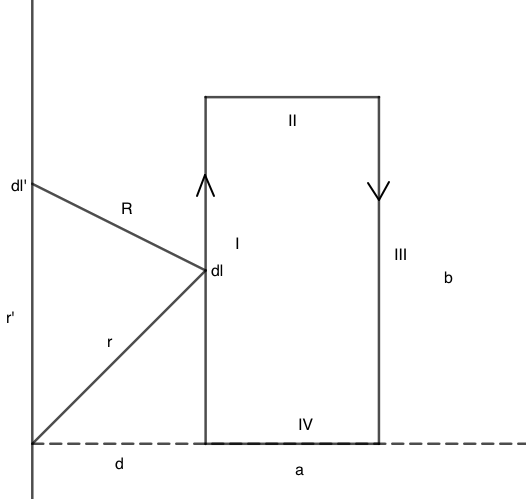
\includegraphics[scale=0.4]{13-4.png}}
            \caption{Drawing for Wangsness 13-4}
        \end{figure}
        \subsubsection{Wangsness 14-7}
        $\mathbf{R} = \mathbf{r}-\mathbf{r}'$, where $\mathbf{r} = z\hat{\mathbf{z}}$ and $\mathbf{r}' = a\cos(\phi')\hat{\mathbf{x}}+a\sin(\phi')\hat{\mathbf{y}}$. We have $\boldsymbol{d\ell}' = ad\varphi' \hat{\boldsymbol{\upvarphi}}$. Putting this together, we have $\mathbf{R} = z\hat{\mathbf{z}} - a(\cos(\phi')\hat{\mathbf{x}}+\sin(\phi')\hat{\mathbf{y}})$. So:
        \begin{align*}
            \mathbf{B} &= \frac{\mu_0 I'}{4\pi}\int \frac{\boldsymbol{d\ell}\times \mathbf{R}}{R^3} = \frac{\mu_0I'}{4\pi} \int_{-\alpha}^{\alpha} \frac{ad\phi' \hat{\boldsymbol{\upvarphi}}\times (z\hat{\mathbf{z}}-a\cos(\phi')\hat{\mathbf{x}}-a\sin(\phi')\hat{\mathbf{y}})}{(z^2+a^2)^{3/2}}\\
            &= \frac{\mu_0 I'a}{4\pi(z^2+a^2)^{3/2}}\int_{-\alpha}^{\alpha} (-\sin(\phi')\hat{\mathbf{x}}+\cos(\phi')\hat{\mathbf{y}})\times (-a\cos(\phi')\hat{\mathbf{x}}-a\sin(\phi')\hat{\mathbf{y}}+z\hat{\mathbf{z}})d\phi'\\
            &= \frac{\mu_0 I'a}{4\pi (z^2+a^2)^{3/2}}\int_{-\alpha}^{\alpha} (z\cos(\phi')\hat{\mathbf{x}}+z\sin(\phi')\hat{\mathbf{y}}+a\hat{\mathbf{z}})d\phi'
        \end{align*}
        Sine is an odd function, and the limit is over a symmetric interval, and thus the $\hat{\mathbf{y}}$ component is zero. So we have:
        \begin{equation*}
            \mathbf{B} = \frac{\mu_0 I' a}{2\pi (z^2+a^2)^{3/2}}\big(z\sin(\alpha)\hat{\mathbf{x}}+a\alpha \hat{\mathbf{z}}\big)    
        \end{equation*}
        \subsubsection{Wangsness 14-15}
        The force on $q$ is given by $\mathbf{F} = q\mathbf{v}\times \mathbf{B}$. We first get $\mathbf{B}$ at $q$. $\mathbf{B} = \frac{\mu_0}{4\pi} \int \frac{I' d\ell' \times \hat{\mathbf{r}}}{R^2}$. For this problem, $\mathbf{R} = -\rho' \hat{\boldsymbol{\uprho}}$. We need only compute the integral along paths $I$ and $III$, for along $II$ and $IV$ we have that $\mathbf{d\ell}$ and $\mathbf{R}$ are parallel. So, we have $\mathbf{B} = \frac{\mu_0}{4\pi} \int_{0}^{\pi} \frac{I'(-ad\phi' \hat{\boldsymbol{\upvarphi}})\times (-a\hat{\boldsymbol{\uprho}})}{a^3}+ \frac{\mu_0}{4\pi} \int_{0}^{\pi} \frac{I'(bd\phi' \hat{\boldsymbol{\upvarphi}})\times (-b\hat{\boldsymbol{\uprho}})}{b^3} = \frac{\mu_0 I'}{4} \frac{b-a}{ab} \hat{\mathbf{z}}$. The force is $\mathbf{F} = qv\hat{\mathbf{y}} \times \frac{\mu_0 I}{4} \frac{b-a}{ab} \hat{\mathbf{z}} = \frac{qv\mu_0 I'}{4} \frac{b-a}{ab} \hat{\mathbf{x}}$
        \begin{figure}[htbp]
            \centering
            {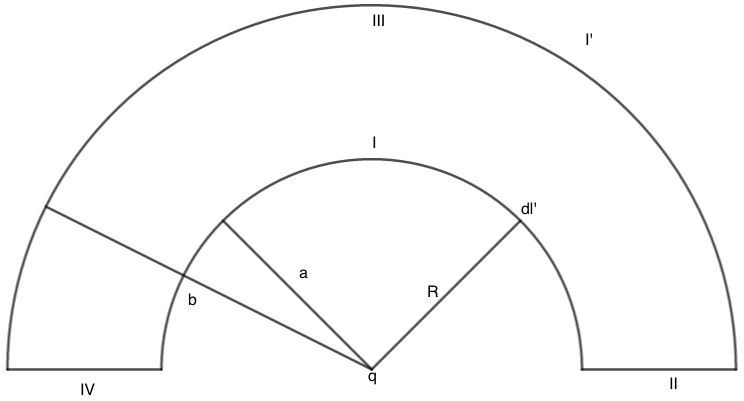
\includegraphics[scale=0.4]{14-15.png}}
            \caption{Drawing for Wangsness 14-15}
        \end{figure}
\end{document}